\chapter{Grundlagen Linux} \label{sec:grund}
Zu Beginn sollen einige Grundlagen näher erläutert werden, die für die Erstellung der Arbeit essenziell waren.

\section{Linux - Kernel und Userspace}\label{sec:linux}
Da das Zielsystem auf Linux läuft, soll zunächst dieses Betriebssystem betrachtet werden. 
Im Herbst 1991 wurde die erste Version des Systems von Linus Torvalds veröffentlicht und der Gründer kümmert sich, mit Unterstützung, weiterhin um die Entwicklung des frei verfügbaren Betriebssystems. \citep[S. 53f.]{plotner2012linux}
 
Der Name Linux bezeichnet dabei eigentlich nur den Kern des Systems, auch Kernel genannt. Zusätzlich benötigt man noch System- und Anwendersoftware. Oft wird dieser Teil als Userspace zusammengefasst. \citep[S. 46]{plotner2012linux} 

Der Kernel hat verschiedene Aufgaben. Unter anderem ist er für die Prozess- und die Speicherverwaltung sowie das Gerätemanagement zuständig. \citep[S. 234]{schroder2009embedded} 
%überprüft am 3.12.

Im Normalfall hat der Nutzer aus dem Userspace keinen direkten Zugriff auf die Kernelfunktionen und die Hardware. Nur über Systemaufrufe, auch Syscalls, hat ein Programm im Userspace die Möglichkeit, Änderungen an der Hardware zu kommunizieren beziehungsweise bestimmte Funktionen im Kernel zu nutzen. \citep[S. 124]{plotner2012linux} 
Der Kernel stellt somit die Brücke zwischen der Hardware und dem Benutzer dar.


\section{\acl{ioctl}}\label{sec:ioctl_t}
Um ein zuverlässig arbeitendes Betriebssystem zu gewährleisten, müssen die Speicherbereiche des Kernel und des Userspace voneinander getrennt sein. \citep[S. 233]{schroder2009embedded} %überprüft am 3.12.

Damit entsteht die Notwenigkeit, zwischen Userspace und Kernel aktiv Daten auszutauschen. Die Anwendungen im Userspace können über das sogenannte Systemcall Interface auf die Funktionen im Kernel zugreifen. In einer Struktur vom Typ \textit{file\_operations} wird die Schnittstelle zu einem Treiber vorgegeben. In dieser Struktur werden treiberabhängige Funktionszeiger gespeichert. \citep[S. 249]{schroder2009embedded} %überprüft am 3.12.

Im Folgenden soll lediglich der Zeiger auf das \acf{ioctl} betrachtet werden, da dieser im weiteren Teil der Arbeit eine wichtige Rolle spielt.
Durch die \ac{ioctl} Methode wird dem Programmierer ein flexibles Werkzeug zur Verfügung gestellt. 


\begin{lstfloat}
\begin{lstlisting}
int (*ioctl) (struct inode *node, struct file *instanz, unsigned int cmd, unsigned long arg);
\end{lstlisting}
\captionof{code}{Funktionsdeklaration des \ac{ioctl} in der file\_operations Struktur \citep[S. 249f.]{schroder2009embedded}} %überprüft am 3.12.
\end{lstfloat}

Über den \textit{node} wird der \gls{dateideskriptor} und über \textit{instanz} ein Zeiger auf die Treiberinstanz an den Funktionszeiger übergeben. Das Kommando wird durch eine Nummer widergespiegelt und ist in der Funktionsdeklaration als \textit{cmd} zu finden. Das optionale Argument \textit{arg} wird als Zeiger auf eine Dateistruktur, welche kopiert werden soll, angegeben. \citep[S. 249f.]{schroder2009embedded} %überprüft am 3.12.


Mit den Übergabeparametern und dem Dateideskriptor wird die Funktion dann in Anwendungen im Userspace aufgerufen, im Kernel werden die Daten weiterverarbeitet und wieder zurückgegeben.

\section{Datenaustausch zwischen Kernel und Userspace}
Durch die Notwendigkeit von getrennten Speicherbereichen des Kernels und des Userspaces, wie im vorausgegangen Kapitel erläutert, wird der Datenaustausch zwischen den beiden Ebenen natürlich schwieriger. Durch \textit{copy\_from\_user} beziehungsweise \textit{copy\_to\_user} stehen im Linux-Kernel zwei Funktionen als hilfreiche Werkzeuge für diesen Austausch zu Verfügung. %todo quelle!


\begin{lstfloat}
\begin{lstlisting}
unsigned long copy_from_user(void *to, const void *from, unsigned long num);
unsigned long copy_to_user(void *to, const void *from, unsigned long num);
\end{lstlisting}
\captionof{code}{\label{code:copy}Vereinfachte Funktionsdeklaration aus \cite[uaccess.h, Zeile 140ff.]{linuxsourceinclude}} %überprüft am 3.12.
\end{lstfloat}

Die Hauptaufgabe beider Funktionen ist das Kopieren von Daten, aber zusätzlich werden die übergebenen Speicherbereiche auf Gültigkeit überprüft. 
In \textit{copy\_from\_user} (siehe Codeausschnitt~\ref{code:code}) werden die Daten ab \textit{from} aus dem Userspace mit der Größe von \textit{num} Bytes an die Stelle \textit{to} in den Kernel kopiert.
Analog arbeitet das Gegenstück \textit{copy\_to\_user}. Hier gibt \textit{from} allerdings die Speicherstelle im Kernel an und somit ist \textit{to} die Stelle im Userspace.
Im Erfolgsfall geben beide Funktionen 0 zurück, andernfalls wird die Anzahl der nicht kopierten Bytes zurückgegeben. \citep[S. 250f.]{schroder2009embedded}%überprüft am 3.12.

\section{Plattformtreiber}\label{sec:plat_t}
Gerätetreiber sind unter Linux im Kernel angesiedelt. Eigene Treiber werden hierzu meist modular entwickelt und nicht fest in den Kernel integriert. Allerdings muss auch der Programmierer bei den nachgeladenen Kernelmodulen auf die korrekte Nutzung des Speicherplatzes achten, da diese Module ebenfalls im Kernel laufen und somit ein Zugriffsfehler schwerwiegende Folgen hätte. \citep[S. 231ff.]{schroder2009embedded}%überprüft am 3.12.

Es gibt im Kernel verschiedene Treiberarten, z.B. den Plattformtreiber und den \ac{pci}-Treiber. Bei letzterem kann das Gerät an einem \ac{pci} Bus mitteilen, von welchem Typ es ist und welchen Speicherbereich es hat. Anderen Geräten ist dies nicht möglich, dann muss dem Kernel mitgeteilt werden, dass die Hardware vorhanden ist. Für diesen Fall werden Plattformtreiber verwendet. \cite{corbet2005linux}

Damit die Treiber richtig funktionieren gibt es einige Bestandteile, die in jedem Modul wiederzufinden sind. Standardmäßig wird die Registrierung von Treiber und Gerät an unterschiedlichen Teilen des Programms ausgeführt. \cite{corbetplatform} %überprüft am 3.12.




Jedes Kernelmodul besitzt mindestens eine \textit{init} und \textit{exit} Funktion. Hierzu gibt es eigene Makros, in welchen die Funktionen übergeben werden und somit den Kernel mit dem Treiber bekannt machen. Der Aufruf ist dann entweder beim Kernelboot bzw. beim Laden oder beim Entfernen des Treibers platziert. \cite[module.h, Zeile 79ff.]{linuxsourceinclude}
%überprüft am 3.12.


\begin{lstfloat}
\begin{lstlisting}
struct platform_driver {
	int (*probe)(struct platform_device *);
	int (*remove)(struct platform_device *);
	void (*shutdown)(struct platform_device *);
	int (*suspend)(struct platform_device *, pm_message_t state);
	int (*resume)(struct platform_device *);
	struct device_driver driver;
	const struct platform_device_id *id_table;
	bool prevent_deferred_probe;
};
\end{lstlisting}
\captionof{code}{\label{code:platform_driver}platform\_driver Struktur in \cite[platform\_device.h, Zeile 184ff.]{linuxsourceinclude}}%überprüft am 3.12.
\end{lstfloat}

Beim Laden des Treibers wird eine \textit{platform\_driver} Struktur übergeben. In dieser Struktur sind Zeiger auf die Funktionen gespeichert, die beim Erzeugen oder Löschen einer Instanz benötigt werden.  
In dieser Arbeit werden lediglich die \textit{probe} und \textit{remove} Funktionszeiger betrachtet. Beim Registrieren einer Instanz wird die Funktion hinter dem \textit{probe} Zeiger aufgerufen und analog beim Auflösen die \textit{remove} Funktion.\cite{corbetplatform}  %überprüft am 3.12.

%todo umformulieren & kapitel zitieren
Beim Anlegen der Instanz kann ein Zeiger auf eine Struktur übergeben werden, in welchem Daten gespeichert sind. In der \textit{probe} Funktion sind somit spezielle Daten für ein entsprechendes Gerät vorhanden. \cite{corbetplatform} %überprüft am 3.12.

\section{\acl{mfd}}\label{sec:mfd_t}
Normalerweise wird lediglich ein Gerät angelegt, ohne weitere Unterteilungen vorzunehmen. Es ist allerdings möglich, dass ein Hardwareblock mehr als eine Funktionalität hat. Damit das gleiche Gerät in mehreren Untersystemen registriert werden kann, muss die Möglichkeit bestehen, es als \ac{mfd} anzulegen. \cite{bellonimfd} %überprüft am 3.12.\\ 

Auf der Abbildung~\ref{fig:mfd} sieht man die Beziehung zwischen dem Elterngerät (links) und den untergeordneten Geräten (rechts), die jeweils verschiedene Funktionalitäten haben können.

\begin{figure}[!hbtp]
	\centering
	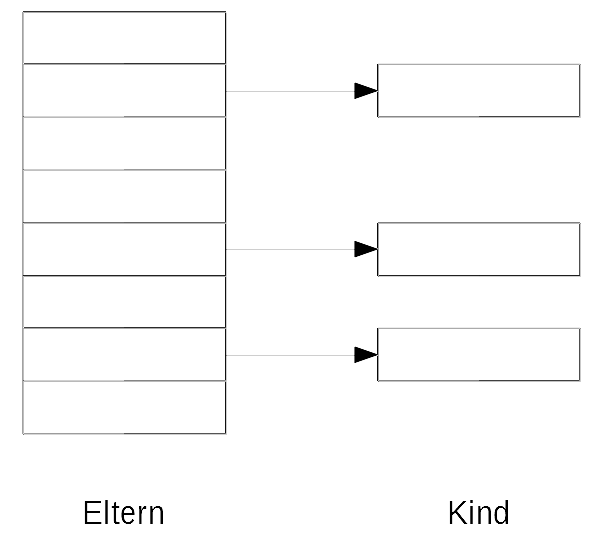
\includegraphics[width = 0.4\linewidth]{pictures/2020-01-10-MFD.png}
	\smallskip
	\caption{Schema zur Funktionsweise des \ac{mfd}}
	\label{fig:mfd}
\end{figure} 


Bevor die Funktion zum Anlegen von \ac{mfd} näher betrachtet wird, sollen zunächst zwei benötigte Strukturen erläutert werden.

\begin{lstfloat}
\begin{lstlisting}
struct resource {
	resource_size_t start;
	resource_size_t end;
	const char *name;
	unsigned long flags;
[...]
	struct resource *parent, *sibling, *child;
};
\end{lstlisting}
\captionof{code}{\label{code:res}Struktur resource in \cite[ioport.h, Zeile 20ff.]{linuxsourceinclude}}%überprüft am 3.12.
\end{lstfloat}

Als erste Struktur wird die \textit{resource} näher betrachtet. Hier werden Parameter für einen Speicherbereich abgelegt, damit auf diesen zugegriffen werden kann. 
Die beiden Parameter sind \textit{start} und \textit{end}. Die beiden Werte legen die Größe und den Ort des Speicherbereichs fest. 
In \textit{name} wird der Name der Datenquelle gespeichert und in der Variable \textit{flags} werden über Definitionen unter anderem der Datentyp und weitere optionale Einstellungen festgelegt.
In den letzten drei Parametern können abhängige Ressources entsprechend ihrem Grad gespeichert werden. \\

%todo id klären
\begin{lstfloat}
\begin{lstlisting}
struct mfd_cell {
	const char		*name;
	int			id;
[...]
/* platform data passed to the sub devices drivers */
	void			*platform_data;
	size_t			pdata_size;	
[...]	
/*
* Device Tree compatible string
* See: Documentation/devicetree/usage-model.txt Chapter 2.2 for details
*/
	const char		*of_compatible;	
[...]	
/*
* These resources can be specified relative to the parent device.
* For accessing hardware you should use resources from the platform dev
*/
	int			num_resources;
	const struct resource	*resources;	
[...]
};
\end{lstlisting}
\captionof{code}{\label{code:mfd_cell}Struktur mfd\_cell in \cite[mfd/core.h, Zeile 29ff.]{linuxsourceinclude}} %überprüft am 3.12.
\end{lstfloat}

Die zweite Struktur wird benötigt um einem \ac{mfd} wichtige Parameter zum Anlegen mitzugeben. Aus diesem Grund werden in der \textit{mfd\_cell} Struktur lediglich die benötigten Parameter betrachtet. 

In der Variable \textit{name} wird der Name des Treibers gespeichert. Durch die \textit{id} bekommt jede Plattformtreiberinstanz beim Allokieren eine spezifische Nummer.
Der \textit{void} Zeiger \textit{platform\_data} ist ein benutzerdefinierter Datenzeiger, welcher an das untergeordnete Gerät weitergereicht wird. Da der Typ variieren kann, wird in \textit{pdata\_size} die zugehörige Datengröße übergeben. 
In der Variable \textit{of\_compatible} wird eine sortierte Liste von strings gespeichert. Beginnend mit dem exakten Namen des Geräts folgt dann eine optionale Liste mit weiteren kompatiblen Geräten. \cite[Zeile 116ff.]{linuxsourcedocu} %überprüft am 3.12. 

Der Zeiger \textit{resources} speichert die zugehörige Ressource ab, bzw. ein Zeiger auf ein Array von Ressourcen. Die Anzahl der abgespeicherten Ressourcen wird in \textit{num\_resources} abgelegt.\\

\begin{lstfloat}
\begin{lstlisting}
extern int devm_mfd_add_devices(struct device *dev, int id, const struct mfd_cell *cells, int n_devs, struct resource *mem_base,int irq_base, struct irq_domain *irq_domain);
\end{lstlisting}
\captionof{code}{\label{code:mfd}Funktionsdeklaration in \cite[mfd/core.h, Zeile 130ff.]{linuxsourceinclude}}%überprüft am 3.12.
\end{lstfloat}

Beim Anlegen eines Untergeräts über \textit{devm\_mfd\_add\_devices} werden mehrere Parameter benötigt. 
Als Erstes wird ein Zeiger auf das übergeordnete Gerät übergeben. Der zweite Übergabeparameter ist die Struktur \textit{mfd\_cell}, wie oben erwähnt, wird diese benötigt, um das anzulegende Gerät näher zu beschreiben.
Durch den Integer \textit{n\_devs} wird die Anzahl der zu registrierenden untergeordneten Geräte angegeben. Dies ist notwendig, da der Parameter \textit{cells} auch ein Array beinhalten kann. 
Die anderen Übergabeparameter werden nicht näher betrachtet, da sie im Folgenden nicht benötigt werden. \cite[Zeile 359ff.]{linuxsourcedriver} %überprüft am 3.12.


In der Funktion ist zusätzlich implementiert, dass beim Entfernen des übergeordneten Gerät alle Untergeräte automatisch aufgelöst werden. \cite[Zeile 356f.]{linuxsourcedriver}%überprüft am 3.12.


%todo warum die Parameter nicht benötigt werden

